%!TeX root=Main Document/Dissertation.tex
\section{Results}

\subsection{Testing the Effect of Sampling Method}
The aim of this test was to identify the effects the sampling method may have had on the genetic algorithm. There are two implementations of sampling method in the program: Roulette Wheel (RW), and Stochastic Universal Sampling (SUS).
Two tests were conducted, using each sampling method respectively, the below factors were standardised between the tests:
\begin{itemize}
\item Number of Generations: 20000
\item Population Generation: Randomised Method
\item Mutation Probability: 1\%
\item Time Step: 1.5 Simulation Seconds per frame
\end{itemize}

\subsubsection{Roulette Wheel Data}

\subsubsection{Stochastic Universal Sampling Data}

\subsubsection{Data Comparison}


\subsection{Testing the Effect of Mutation Probability}
This was a test to identify the affect mutation probability had on the genetic makeup of the flock and to identify the affect it may have on the effectiveness of the genetic algorithm as a whole. This required standardising the tests in each run of the GA, these were:
\begin{itemize}
\item Number of Generations: 5000
\item Population Generation: Randomised Method
\item Selection Type: Stochastic Universal Sampling
\item Time Step: 1.5 Simulation Seconds per frame
\end{itemize}
Keeping these factors controlled across all tests, 10 tests were then produced with different mutation probabilities: 0.5\%, 1\%, 2\%, 3\%, 4\%, 5\%, 10\%, 15\%, 20\%, and 25\%.

\subsubsection{The Effect on Fitness}
Below is the data collected regarding the fitness value of the boids over each generational improvement. This data will shine a light onto the effect the mutation rate has on the boids fitness.

\begin{figure}[H]
	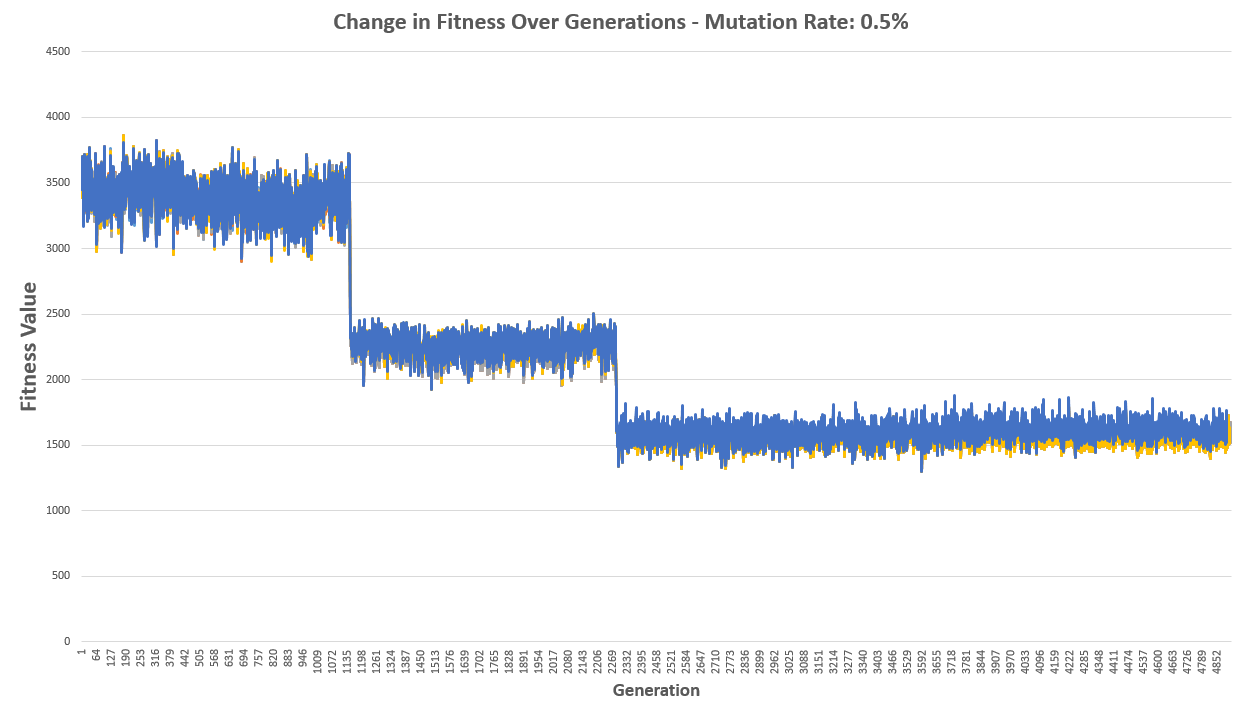
\includegraphics[width=\linewidth]{../Images/05Mutation.png}
	\caption{A graph displaying the fitness each generation with a mutation rate of 0.5\%}
	\label{fig:0.5mutation}
\end{figure}

\begin{figure}[H]
	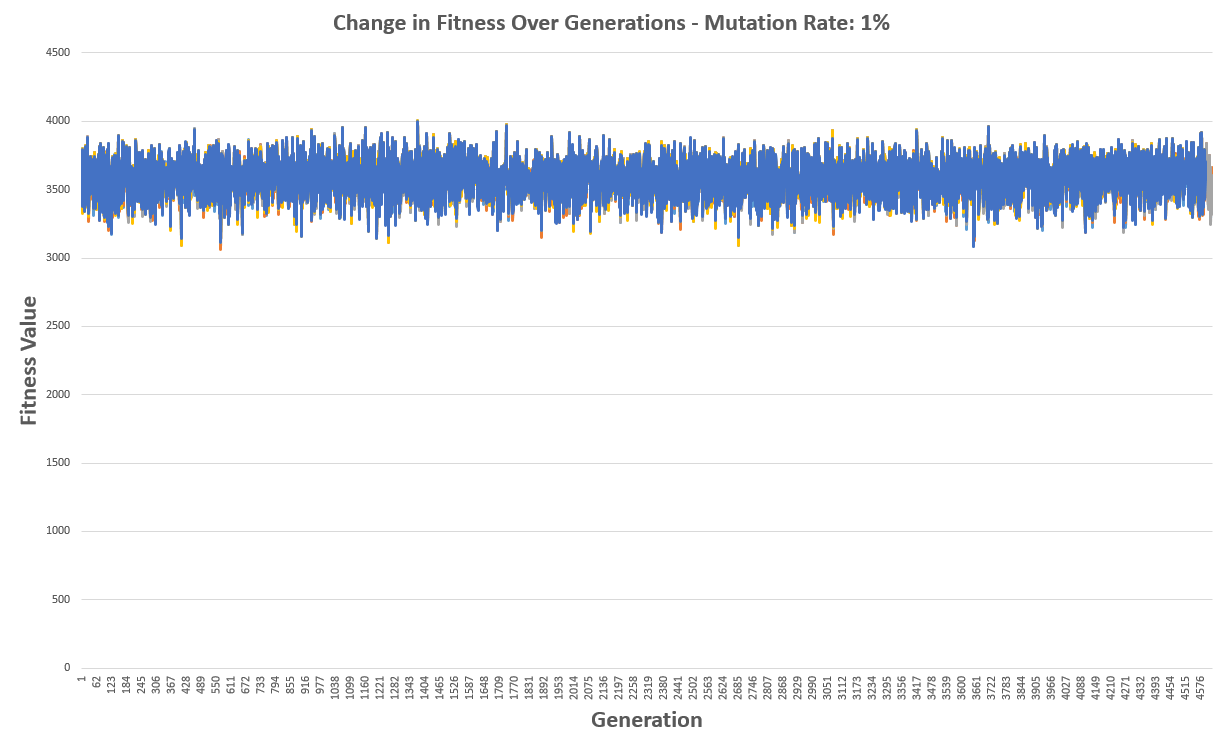
\includegraphics[width=\linewidth]{../Images/1Mutation.png}
	\caption{A graph displaying the fitness each generation with a mutation rate of 1\%}
	\label{fig:1mutation}
\end{figure}

\begin{figure}[H]
	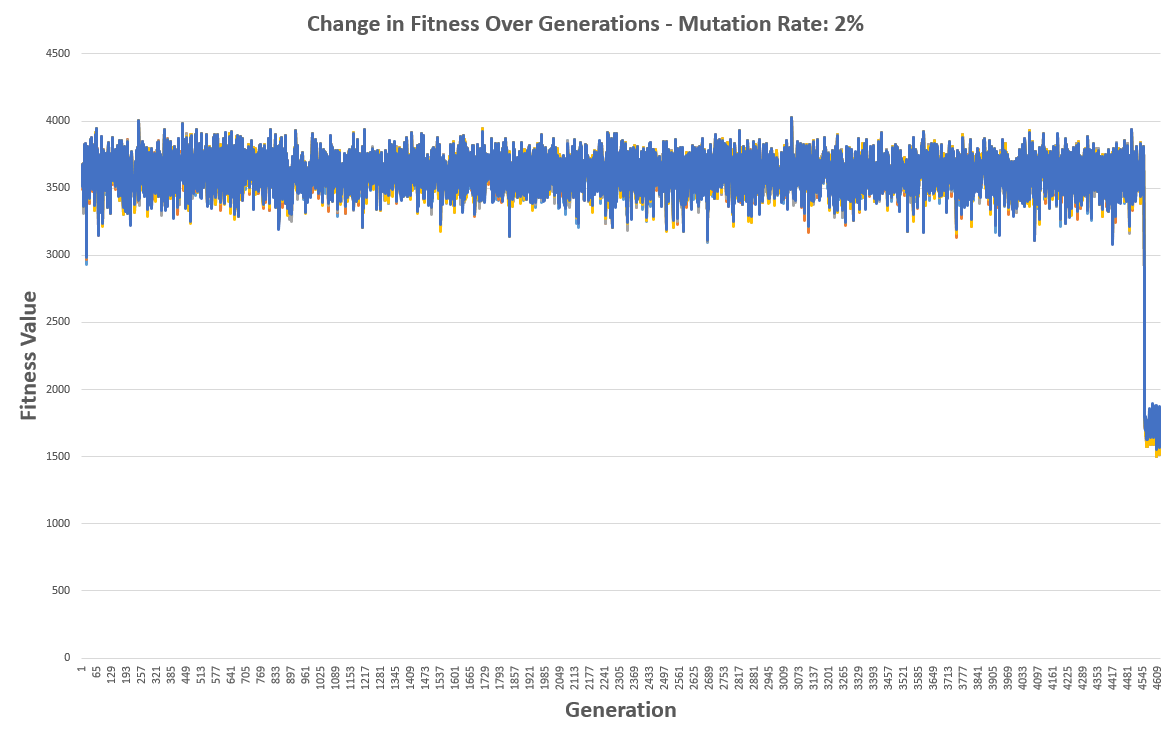
\includegraphics[width=\linewidth]{../Images/2Mutation.png}
	\caption{A graph displaying the fitness each generation with a mutation rate of 2\%}
	\label{fig:2mutation}
\end{figure}

\begin{figure}[H]
	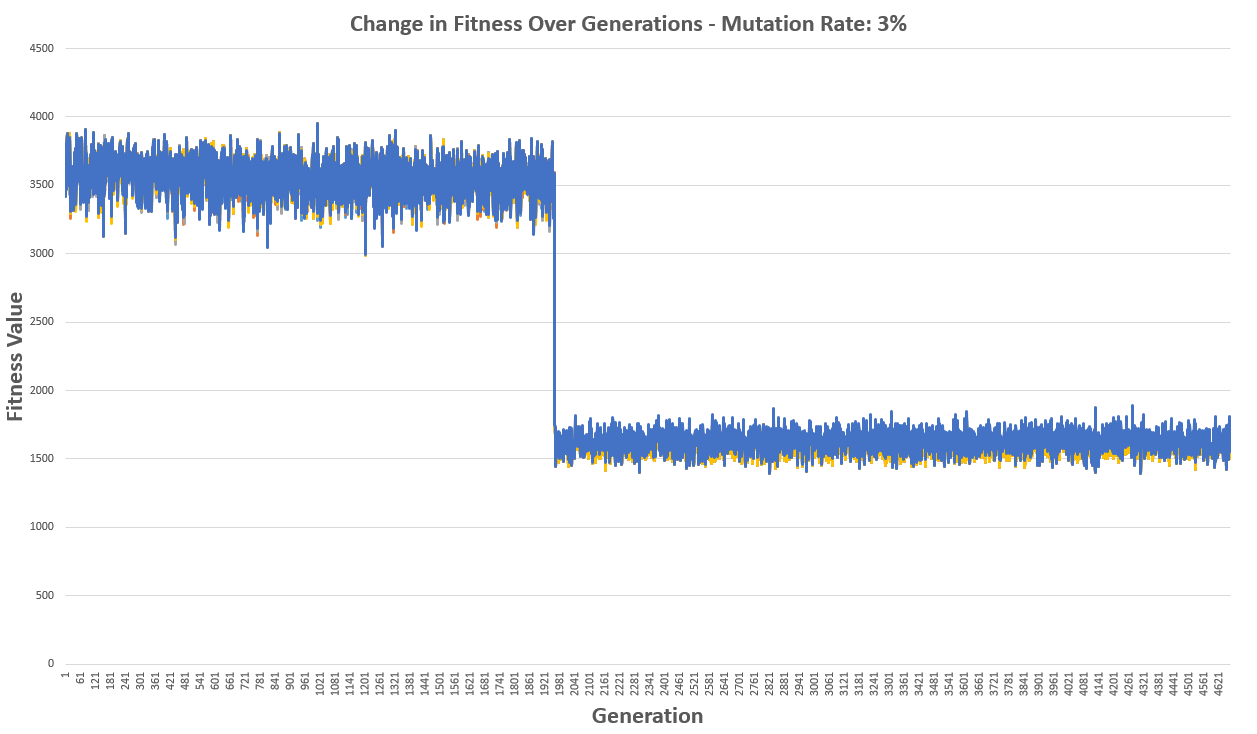
\includegraphics[width=\linewidth]{../Images/3Mutation.png}
	\caption{A graph displaying the fitness each generation with a mutation rate of 3\%}
	\label{fig:3mutation}
\end{figure}

\begin{figure}[H]
	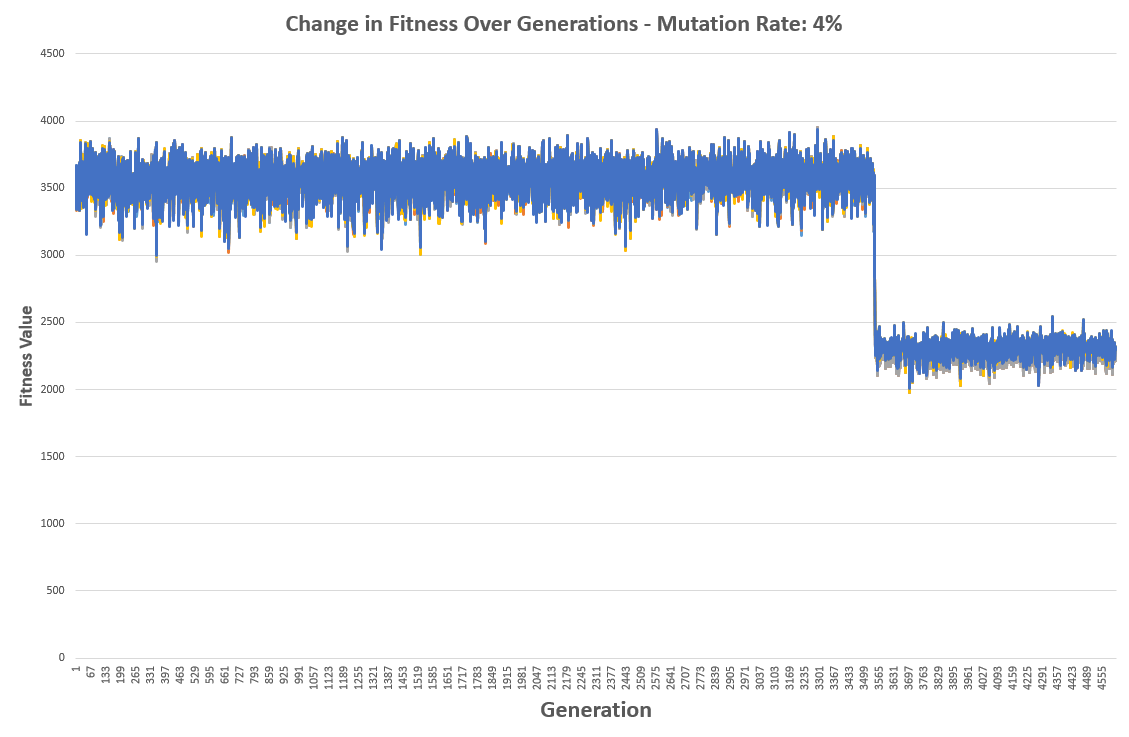
\includegraphics[width=\linewidth]{../Images/4Mutation.png}
	\caption{A graph displaying the fitness each generation with a mutation rate of 4\%}
	\label{fig:4mutation}
\end{figure}

\begin{figure}[H]
	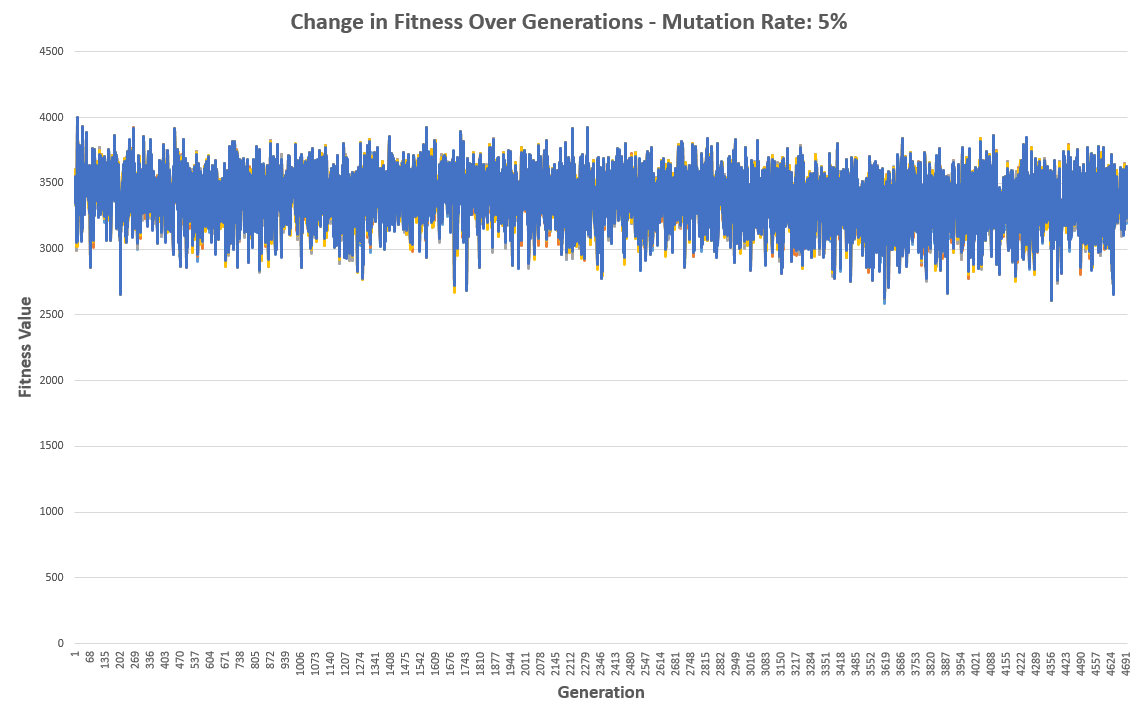
\includegraphics[width=\linewidth]{../Images/5Mutation.png}
	\caption{A graph displaying the fitness each generation with a mutation rate of 5\%}
	\label{fig:5mutation}
\end{figure}

\begin{figure}[H]
	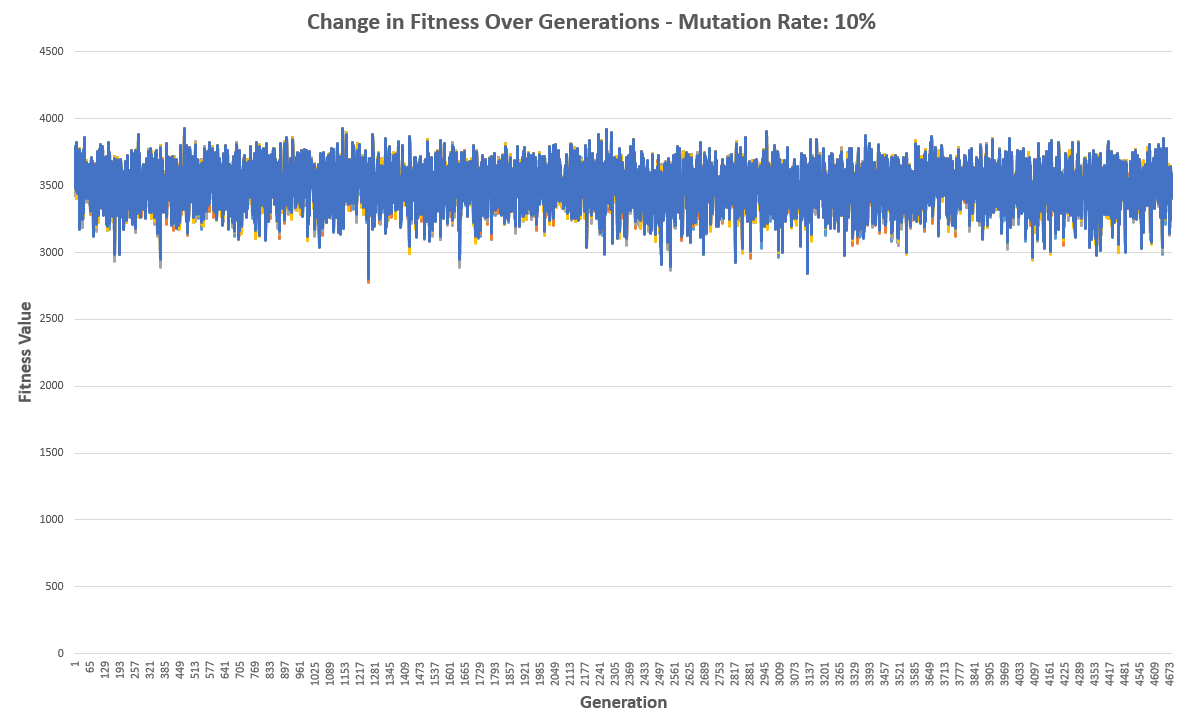
\includegraphics[width=\linewidth]{../Images/10Mutation.png}
	\caption{A graph displaying the fitness each generation with a mutation rate of 10\%}
	\label{fig:10mutation}
\end{figure}

\begin{figure}[H]
	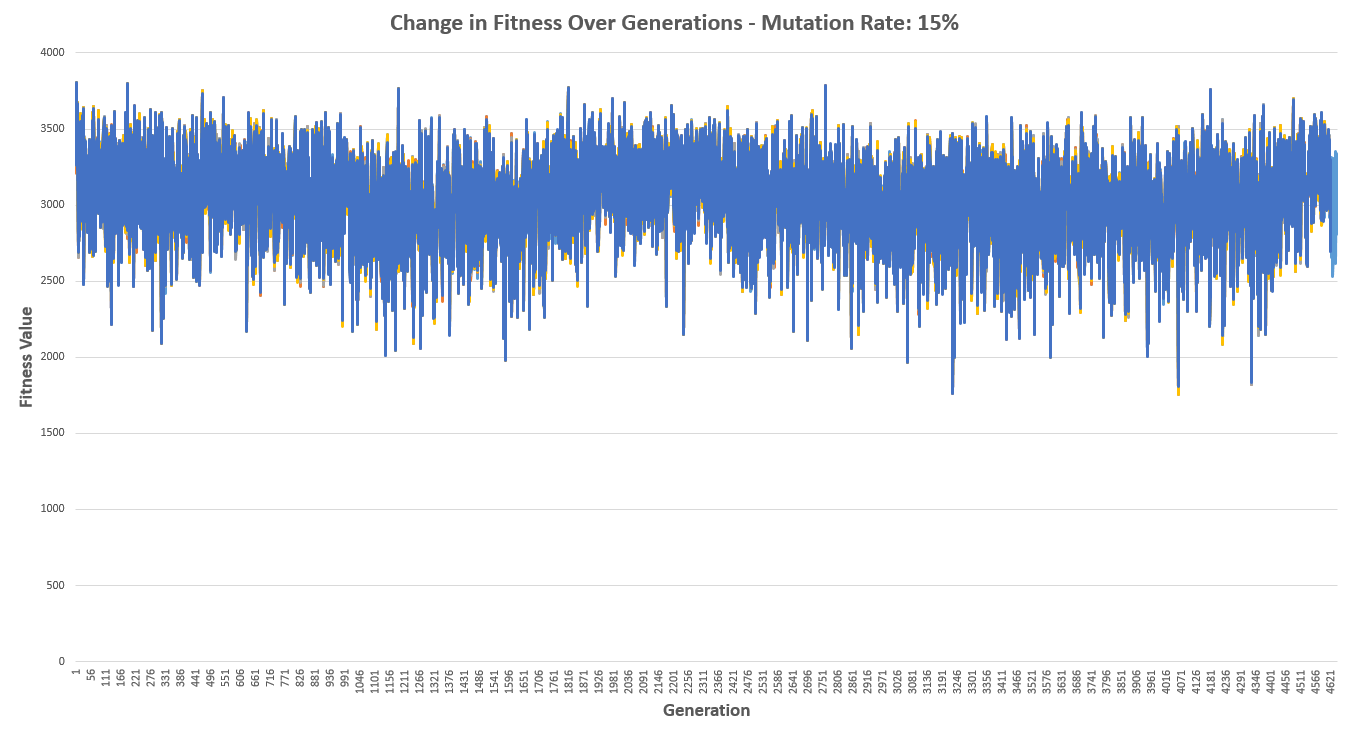
\includegraphics[width=\linewidth]{../Images/15Mutation.png}
	\caption{A graph displaying the fitness each generation with a mutation rate of 15\%}
	\label{fig:15mutation}
\end{figure}

\begin{figure}[H]
	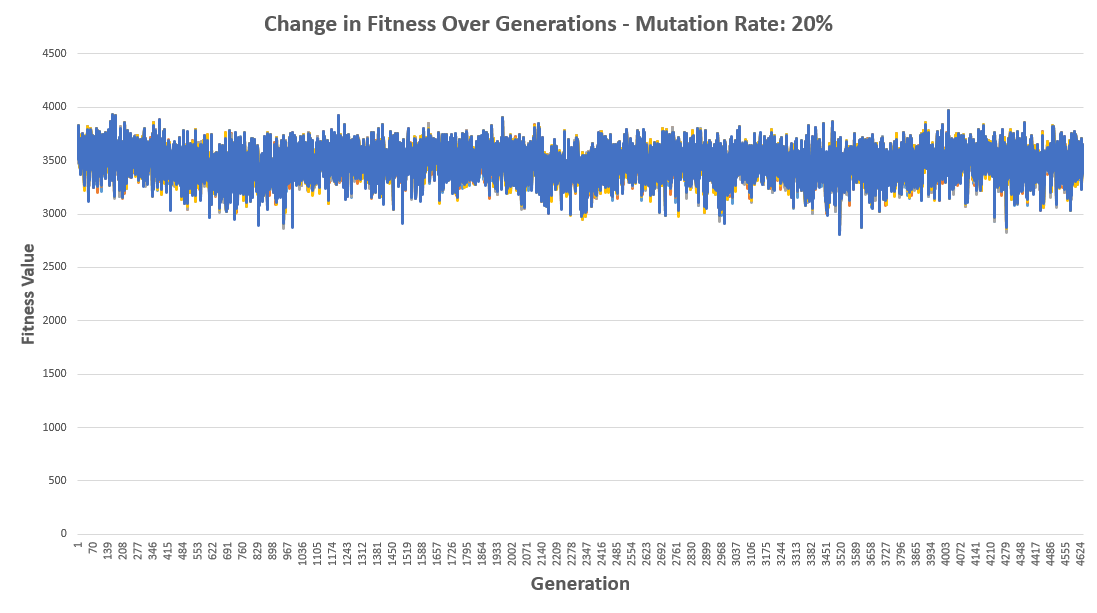
\includegraphics[width=\linewidth]{../Images/20Mutation.png}
	\caption{A graph displaying the fitness each generation with a mutation rate of 20\%}
	\label{fig:20mutation}
\end{figure}

\begin{figure}[H]
	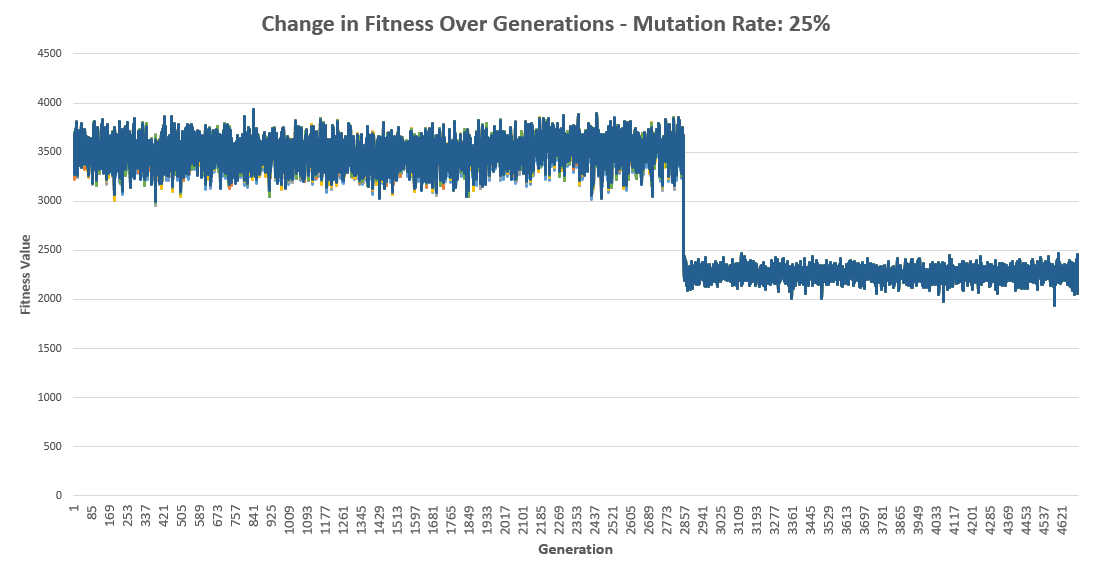
\includegraphics[width=\linewidth]{../Images/25Mutation.png}
	\caption{A graph displaying the fitness each generation with a mutation rate of 25\%}
	\label{fig:25mutation}
\end{figure}



\subsection{Allele Convergence}
Using the data collected from the previous tests, the aim was to analyse the frequency of different alleles to identify the most frequently produced values in the simulation as this may point toward optimal solutions for the boid algorithm. 

\subsection{Genotype Convergence}

\subsection{Phenotype Effects of Common Genotypes}


\subsection{Strategies}
By visually analysing the flocks in action 






















